% ══════════════════════════════════════════════════════════════════════════════
%  CHAPTER 3: ENERGY BUDGET IN THE ΛCDM MODEL
% ══════════════════════════════════════════════════════════════════════════════

\chapter{Energy Budget in the $\Lambda$CDM Model}

% ──────────────────────────────────────────────────────────────────────────────
\section{Density Parameters \& Critical Density}

\subsection{Physics Intuition}

\begin{intuition}
The \emph{critical density} $\rho_\mathrm{crit}$ is the threshold total energy density
at which the universe has exactly flat geometry.
A universe denser than $\rho_\mathrm{crit}$ would be positively curved
and—in the absence of dark energy—would re-collapse in a Big Crunch;
one less dense would be negatively curved and expand forever.
Observations show our universe is within $0.5\%$ of the critical density,
implying either extraordinary initial fine-tuning or a dynamical mechanism such as
cosmological inflation that drove it toward flatness.
\end{intuition}

\subsection{Theory}

\begin{theory}
Define the \textbf{critical density} and dimensionless density parameters:
\begin{equation}
  \rho_\mathrm{crit}(z) = \frac{3H(z)^2}{8\pi G}, \qquad
  \Omega_i(z) = \frac{\rho_i(z)}{\rho_{\mathrm{crit}}(z)}.
\end{equation}
Each component scales with redshift according to its equation of state $w_i$:
\begin{equation}
  \rho_i(z) = \rho_{i,0}(1+z)^{3(1+w_i)}.
\end{equation}

The flatness condition $\sum_i \Omega_i = 1$ (for $k=0$) is equivalent to
$\Omega_\mathrm{m,0} + \Omega_{\Lambda} + \Omega_\mathrm{r,0} = 1$ in a universe
containing only matter, radiation, and a cosmological constant.
A non-zero spatial curvature contributes a term
$\Omega_{k} = -kc^2/(a_0 H_0)^2$ to the sum, shifting it away from unity.
\end{theory}

\begin{importantnote}
  The density parameter $\Omega_k$ for curvature is \emph{not} a physical energy
  component; it is a bookkeeping term that ensures the Friedmann equation takes the
  compact form $\sum_i\Omega_i + \Omega_k = 1$.
  Do not confuse it with matter or radiation density: $\Omega_k < 0$ corresponds to
  positive curvature ($k = +1$), and $\Omega_k > 0$ to negative curvature ($k = -1$).
\end{importantnote}

\begin{foundation}
\textbf{Derivation of $\rho_\mathrm{crit}$ from the Friedmann equation.}
Recall the first Friedmann equation (for a flat or curved universe):
\[
  H^2 = \left(\frac{\dot a}{a}\right)^2
      = \frac{8\pi G}{3}\rho_\mathrm{tot} - \frac{kc^2}{a^2}.
\]
Setting the spatial curvature to zero ($k = 0$) defines the critical total energy
density required to achieve exact flatness:
\[
  H^2 = \frac{8\pi G}{3}\rho_\mathrm{crit}
  \implies
  \rho_\mathrm{crit} = \frac{3H^2}{8\pi G}.
\]
For an arbitrary universe with $\rho_\mathrm{tot} \neq \rho_\mathrm{crit}$,
dividing both sides of the Friedmann equation by $H^2$ gives
\[
  1 = \frac{\rho_\mathrm{tot}}{\rho_\mathrm{crit}} - \frac{kc^2}{a^2 H^2}
  \equiv \Omega_\mathrm{tot} + \Omega_k,
\]
showing that $\Omega_k \equiv -kc^2/(aH)^2$ exactly accounts for the departure
from flatness.
\end{foundation}

\begin{remark}
  The word ``critical'' refers to the fact that $\rho_\mathrm{crit}$ is the
  \emph{threshold} between an open and a closed universe in the absence of a
  cosmological constant.  In modern $\Lambda$CDM cosmology this geometric
  interpretation is supplemented by the role dark energy plays: even with
  $\Omega_k \approx 0$, the universe accelerates rather than re-collapsing.
\end{remark}

\subsection{Question Examples}

\begin{example}{Computing Critical Density Today}{}
Calculate $\rho_\mathrm{crit}$ at $z=0$ using
$H_0 = 67.4\,\mathrm{km\,s^{-1}\,Mpc^{-1}}$.
Express your answer in $\mathrm{kg\,m^{-3}}$ and in protons per cubic metre.

\medskip\textbf{Solution.}\quad
Convert to SI: $H_0 = 67400/(3.086\times10^{22})\,\mathrm{s^{-1}}
= 2.18\times10^{-18}\,\mathrm{s^{-1}}$.
Then $\rho_\mathrm{crit} = 3H_0^2/(8\pi G)
\approx 8.5\times10^{-27}\,\mathrm{kg\,m^{-3}}$.
Dividing by $m_p = 1.67\times10^{-27}\,\mathrm{kg}$ gives
$\approx 5.1$ protons per cubic metre—an astonishingly sparse universe.
\end{example}

\subsection{Extra}

\begin{extra}
The flatness of the universe is closely tied to inflationary cosmology:
a brief period of exponential expansion at $t \sim 10^{-36}\,\mathrm{s}$
stretches any initial curvature to imperceptibly small values, predicting
$|\Omega_k| \ll 1$ today.
This prediction was confirmed to $<0.5\%$ by the positions of acoustic peaks
in the Planck CMB power spectrum—one of inflation's most compelling successes.
\end{extra}

% ──────────────────────────────────────────────────────────────────────────────
\section{The Flat $\Lambda$CDM Model}

\subsection{Physics Intuition}

\begin{intuition}
The $\Lambda$CDM model is the standard model of cosmology, successfully describing
observations from the CMB to the large-scale structure of galaxies.
Its dominant components are: baryonic matter ($\sim5\%$), cold dark matter
($\sim27\%$), and a cosmological constant $\Lambda$ (dark energy, $\sim68\%$).
Despite its observational success, the physical nature of both dark matter and
dark energy remain unknown—arguably the two greatest open questions in
fundamental physics today.
\end{intuition}

\subsection{Theory}

\begin{theory}
In the \textbf{flat $\Lambda$CDM} model ($\Omega_k=0$,
$\Omega_\mathrm{m,0}+\Omega_{\Lambda}+\Omega_\mathrm{r,0}=1$):
\begin{equation}
  \frac{H(z)^2}{H_0^2}
    = \Omega_{\mathrm{m},0}(1+z)^3
    + \Omega_{\mathrm{r},0}(1+z)^4
    + \Omega_\Lambda.
  \label{eq:lcdm_hubble}
\end{equation}

Current Planck~2018 best-fit values:
\begin{equation*}
  \Omega_\mathrm{m,0} \approx 0.315, \quad
  \Omega_\Lambda \approx 0.685, \quad
  \Omega_\mathrm{r,0} \approx 9.2 \times 10^{-5}.
\end{equation*}
The cosmological constant $\Lambda$ (or equivalently, dark energy with equation of state
$w_\Lambda = -1$) constitutes roughly two-thirds of the universe's energy budget today.
Its value and physical interpretation remain deeply mysterious \citep{Carmeli_2001}.

The energy budget evolves dramatically with redshift.
At early times radiation dominated ($\rho_\mathrm{r}\propto a^{-4}$ dilutes fastest);
the \emph{matter--radiation equality} at $z_\mathrm{eq}\approx3400$ marks the transition
to the matter-dominated era that shaped large-scale structure.
Dark energy overtook matter around $z\approx0.4$, initiating the current
phase of accelerated expansion.
As $z\to-1$ (far future), $H(z)\to H_0\sqrt{\Omega_\Lambda}$—the universe
approaches an exponential de~Sitter expansion.
\end{theory}

\subsection{Question Examples}

\begin{example}{Age of the Universe in Flat $\Lambda$CDM}{}
Using Planck~2018 parameters, evaluate the age integral
$t_0 = \int_0^\infty dz/[(1+z)H(z)]$
and show that it gives $t_0 \approx 13.8\,\mathrm{Gyr}$.

\medskip\textbf{Solution.}\quad
The lookback-time integral is:
\begin{equation}
  t_0 = \int_0^\infty \frac{dz}{(1+z)\,H(z)},
\end{equation}
with $H(z)$ from Eq.~\eqref{eq:lcdm_hubble}.
Substituting Planck~2018 values and numerically integrating (e.g.\ with
\texttt{scipy.integrate.quad}) yields $t_0 \approx 13.8\,\mathrm{Gyr}$,
consistent with the ages of the oldest globular clusters ($12$--$13\,\mathrm{Gyr}$).
\end{example}

\subsection{Extra}

\begin{extra}
The \emph{Hubble tension}—the $\sim5\sigma$ discrepancy between early-universe
(CMB-based, $H_0\approx67.4$) and late-universe (Cepheid/SN~Ia distance ladder,
$H_0\approx73$) measurements of $H_0$ in units of
$\mathrm{km\,s^{-1}\,Mpc^{-1}}$—remains unresolved.
Proposed extensions to $\Lambda$CDM include early dark energy, self-interacting
dark matter, or extra relativistic species.
Whether this tension signals new physics or unaccounted systematics is one of
the most actively debated questions in observational cosmology.
\end{extra}

\clearpage

% ──────────────────────────────────────────────────────────────────────────────
\section{Energy Budget Evolution}

\subsection{Visualizing the Energy Density}

\begin{figure}[htbp]
  \centering
  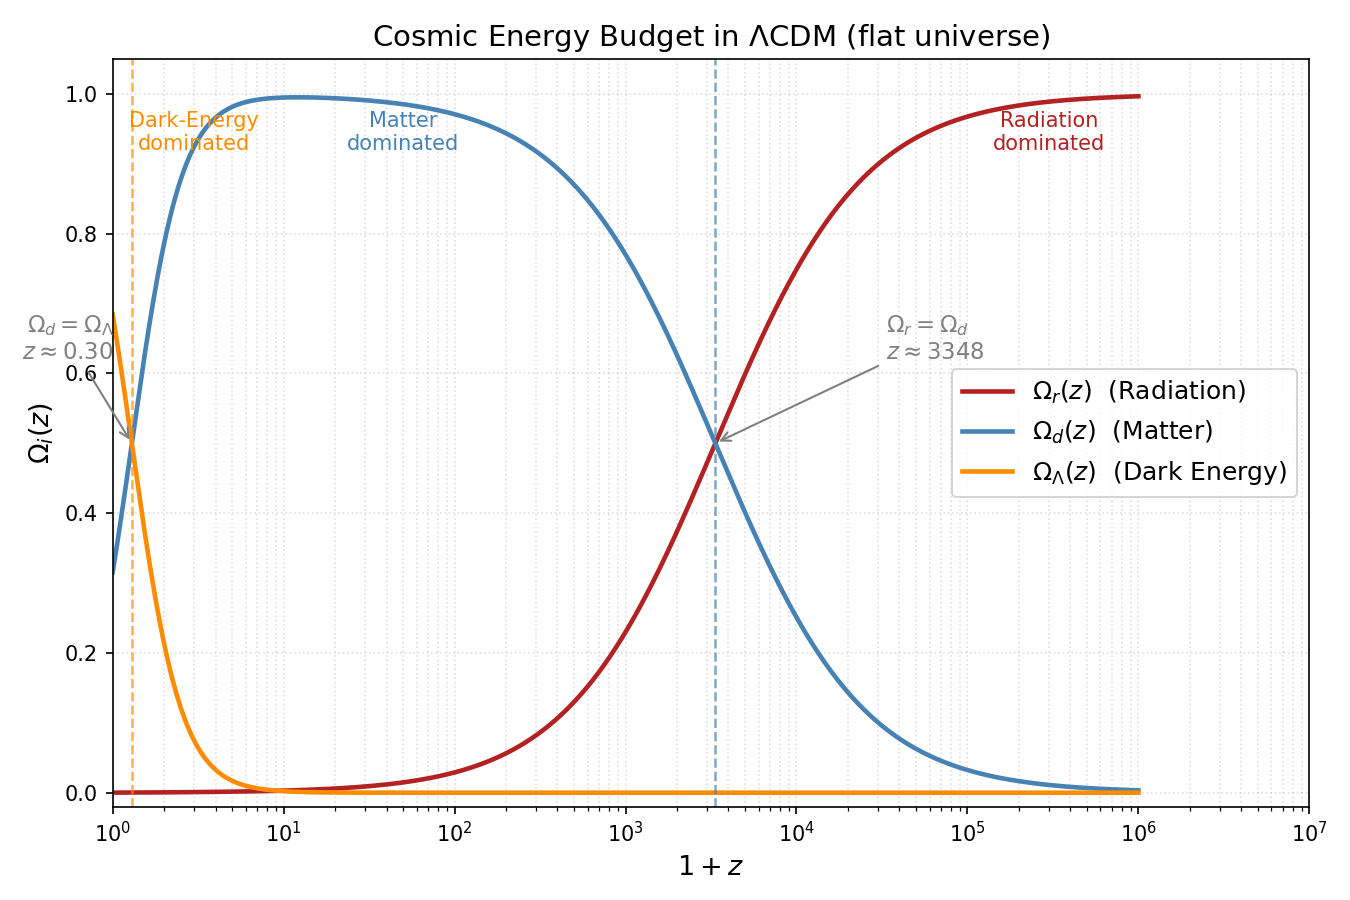
\includegraphics[width=0.85\textwidth]{images/lcdm_energy_budget.png}
  \caption{%
    \textbf{Evolution of energy density components in the flat $\Lambda$CDM model.}
    The figure shows how the fractional energy density (normalized to critical density)
    of matter (dark and baryonic), radiation, and dark energy evolve with redshift $z$.
    At early times ($z \gg 1$), radiation dominated; at intermediate times, matter dominated;
    and at late times ($z \lesssim 1$), dark energy becomes dominant.
    \label{fig:lcdm_budget}
  }
\end{figure}

\begin{extra}
The visualization of energy budget components provides crucial insights into cosmic evolution.
Early universe physics was radiation-dominated, while the matter-dominated era shaped structure
formation and galaxy evolution. The recent transition to dark-energy domination (around $z\sim 0.7$)
explains the observed cosmic acceleration detected through Type Ia supernovae observations
\citep{Carmeli_2001}.
\end{extra}
